\documentclass[12pt, a4paper]{article}

\usepackage[utf8]{inputenc}
\usepackage{graphicx} % to embed images
\usepackage{hyperref} % to link the table of contents
\usepackage{subcaption} %complex images
\usepackage{placeins} %floating
%\usepackage{pdflscape} %to allow single pages in landscape mode
\usepackage[top=1.25in, bottom=1.25in, left=1in, right=1in]{geometry}
\usepackage{verbatim} % include raw text file (for Alloy)
\usepackage[export]{adjustbox}

\title{Requirement Analysis and Specification Document}
\date{2017-10-26}
\author{
	Leonardo Bisica
	\and
	Alessandro Castellani
	\and
	Michele Cataldo
}

\begin{document}
	%%% titlepage %%%
	\begin{titlepage}
		\centering
		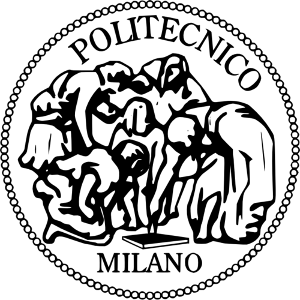
\includegraphics[width=5cm]{img/polimi_logo.png} % also works with logo.pdf
		\vfill
		{\bfseries\Large
			Travlendar+\\
			Requirement Analysis and Specification Document
			Version 0.1\\
			\vskip4cm
			Leonardo Bisica\\
			Alessandro Castellani\\
			Michele Cataldo\\
		}
		\vfill
		\vfill
	\end{titlepage}

	%%% table of contents %%%
	\tableofcontents
	
	\newpage
%%% 1 - INTRODUCTION %%%
	\section{Introduction}
		\subsection{Purpose}
		
		This document is the \textit{Requirement Analysis and Specification Document} (from now on RASD) for the information system \textit{Travelandar+}.
		This application aims to help users in their everyday life by organizing their appointments and optimizing their travel means.
		No previous versions of this application have been developed. 
		We’ll start by describing Stakeholders’ aims (Goals), from which we obtain, subsequently, functional and nonfunctional requirements (\textit{Requirements} Section) useful to describe the system.
		In addition we will need two other sections to have a complete overview of the model: \textit{Constraints} Section is going to describe constraints about the system, while \textit{Domain Properties} Section is going to underline the limits forced by the world on our software.
		After having spoken about this first chapter we are going to analyze some scenarios and use cases of the application.
		
		%TODO	
		\subsubsection{Goals}
			\begin{enumerate}
	\item
		[G1] System allows guest user to register with an username ad and a password; to complete the procedure user should confirm by 

	\item
		[G2] System Login

	\item 
		[G3] Registered User can create meetings 
	\item 
		[G4] Registered User can edit meetings
	\item 
		[G5] The application can automatically compute a personalized selection of travel times between appointments to choose from
	\item
		[G6] User can choose a preferred solution among the best ones
	\item
		[G7] The application warns the user if locations are unreachable in the allotted time
	\item
		[G8] Allow users to put constraints on different travel means and limit carbon footprints
	\item
		[G9] The application features additional user’s privileged time spans
	\item
		[G10] The application allows to arrange the trips : tickets for public services
	\item	
		[G11] The application allows the nearest shared vehicle to be found
	\item
		[G12] The application can obtain the position of the device and consequently of its user
		
\end{enumerate}	


		
		\subsection{Scope}
		The aim of this project is to develop \textit{Travlendar+}, a calendar-based mobile application. 
		The main functionality of the system is helping people in scheduling their appointments by taking into account useful, external information regarding traffic, public transportation, weather, and the like. 
		Appointments could be scheduled through the entire region of Lombardy (Italy), and the main Italian cities connected via railway system. There could be several types of work meetings and personal appointments.
		Furthermore the system can help the user by allowing the purchase of public transportation tickets via the mobile application itself, or by reserving a car or a bike of a sharing system (whenever this is possible). In case of bad weather the system should find alternative moving solutions in order to replace walking paths, same goes with strikes and other relevant kinds of information. 
		Naturally, the system will also allow the registration of new users; as for the registration, the system requests both personal and payment information. After the registration succeeds, the user could immediately start scheduling his meetings.
		
		\subsection{Glossary}
			\begin{description}
				\item[User] 
				\begin{itemize}
					\item First name;
					\item Last name; 
					\item Email;
					\item Username;
					\item Password;
					\item Payment information; this in particular includes:
						\begin{itemize}
							\item Credit card owner;
							\item Credit card number;
							\item Credit card expiration date;
							\item CVV number.
						\end{itemize}
				\end{itemize}
				
				\item[Guest] We name 'guests' all the people who are using the interface of the system without being registered or logged in. Guests can't access any functionality of \textit{Travlendar+} except for the registration process and the log in. 
				\item[Operative Zone] We name Operative Zone the area within we can place the location of an event. For the time being the Operative Zone coincide with all the cities and places within italian peninsula that can be reached by simply consulting the Google APIs. Naturally, such an area may be expanded in the future.
				\item[Influence Zone] We name Influence Zone the area within whose borders the mobile application can not only give travel time by car and on foot (the minimum standard given to us by Google APIs) but also where Travlendar+ can rely at least on a single car and bike sharing service. For starting, the Influence Zone will coincide with the city of Milan.
				\item
				\item[Registered User] A registered User is a former guest who inserted his/her own credentials in the system. After previous login, a Registered User can then create events, work on the timetable and ultimately is the end-user of Travlendar+.
				\item[Timetable]
				\item[Vehicle Sharing services/systems and a Shared Vehicle] By vehicle sharing we do not inted referring to a generic 'car-pooling' service. The usage of a shared vehicle may be either one of two types, car or bike sharing. A vehicle within the system operates only within the boundaries and parking zones imposed by its service; it can be picked up by any user registered to its corresponding system, used for the required amount of time (even though a maximum time is always fixed) and then parked in an allowed zone, ready to be picked by up again by another user. Eahc sharing system possesses an individual API			
				\item[Mobile Application] By mobile application we refer to a program conceived for Android and iOS operative systems, based on touch interfaces and able to run on portable devices. The logic of the mobile application is the system.
				\item[Appointment] An appointment is an event well delimited both in time and space, requiring the presence and the direct investment, in our case, of the user who creates it. Appointments fall in two categories : work appointments (that are often referred also as meetings) and personal appointments (the broader set encapsulating all other kinds of appointments, mainly regarding personal and family life)
				\item[Warning] A warning is a notification given by Travlendar+ mobile application to the operating System it is hosted by. It behaves as a standard system notification.
				\item[Travel Logic] By travel logic we refer to the logic that processes the distances and the transportation time within our operative and influcence zones. In the case at hand, in this first implementation, we're going to adopt as Travel Logic the Google Maps APIs.
\end{description}

		
		\subsection{Revision History}
			No revision where done since first edition of this document.
			
		\subsection{Reference Document}
			\begin{itemize}
				\item Specification Document : Mandatory Project Assignments.pdf
				\item -
			\end{itemize}
		
		\subsection{Document Structure}	

%%% 2 - OVERALL DESCRIPTION  %%%
	\newpage
	\section{Overall Description}
		
		\subsection{Product perspective}
			%cose a caso
			
		\subsection{Product functions}
			%Requirement
			
		\subsection{User characteristics}
			%cose a caso 2	
			
		\subsection{Assumptions, dependencies and constraints}
			%si spiega da sola

%%% 3 - SPECIFIC REQUIREMENTS %%%

%TODO creare nuove sottosezioni
		\section{Specific Requirements}
			\subsection{External Interface Requirements}
				\begin{description}
					\item[User Interfaces]
					\item[Hardware Interfaces]
					\item[Software Interfaces]
					\item[Communication Interfaces]
				\end{description}
						
			\subsection{Functional Requirements}
			
			\subsection{Performance Requirements}
			
			\subsection{Design Constraints}
				\begin{description}
					\item[Standards compliance]
					\item[Hardware limitations]
					\item[Any other constraint]
				\end{description}
				
			\subsection{Software System Attributes}
				\begin{description}
					\item[Reliability]
					\item[Availability]
					\item[Security]
					\item[Maintainability]
					\item[Portability]
				\end{description}
			
				

%%% 4 - ALLOY %%%

	\newpage
	\section{Alloy modeling}

	\newpage
	%%% appendix %%%
	\section{Appendix}
		\listoffigures
		\listoftables
		
		\subsection{Used tools}
		For this assignment, we used the following tools:
		
		\begin{description}
			\item [Alloy] We used the alloy tool to write the code and check the models for the specification.
			\item [LaTeX] The group used LaTeX to structure the final document and to help with versioning.
			\item [Github] We leaned on Github for versioning and coordinating synchronized work.
			
		\end{description}
		
		\subsection{Hours of work}
			\begin{description}
				\item[Bisica, Leonardo] around xx hours of work;
				\item[Castellani, Alessandro] around xx hours of work;
				\item[Cataldo, Michele] around xx hours of work.
			\end{description}
			
\end{document}